\documentclass[12pt]{article}

\usepackage[utf8]{inputenc}
\usepackage{fancyhdr}
\usepackage{xcolor,graphicx}
\usepackage{fancyvrb}
\usepackage{tcolorbox}
% Allow hypertext links
\usepackage{hyperref}
\usepackage{ulem}
% Allow better labels and captions management
\usepackage{caption}
\captionsetup[figure]{font=small}
\usepackage{floatrow}
\newcommand*\ruleline[1]{\par\noindent\raisebox{.8ex}{\makebox[\linewidth]{\hrulefill\hspace{1ex}\raisebox{-.8ex}{#1}\hspace{1ex}\hrulefill}}}
\usepackage[%
linewidth=0.5pt,
middlelinecolor= black,
middlelinewidth=0.4pt,
roundcorner=1pt,
rightmargin=-1cm,
skipabove=0pt,
skipbelow=0pt,
leftmargin=-1cm,
innerleftmargin=1cm,
innerrightmargin=1cm,
innertopmargin=0pt,
innerbottommargin=0pt,
]{mdframed}

\hypersetup{
    colorlinks=true,
    linkcolor=blue,
    filecolor=blue,      
    urlcolor=blue,
}

% Allow explicit linebreaks in table items
\usepackage{makecell}
\usepackage{float}

% Allow tables to span page boundaries
\usepackage{longtable}
\setlength{\LTpre}{5pt}
\setlength{\LTpost}{5pt}

\pagestyle{fancy}

%\lhead{Parallel Computing with LMGC90}
\chead{}
\rhead{} 
\lfoot{}
\cfoot{}
\rfoot{\hfill \thepage}
\renewcommand{\headrulewidth}{0pt}

\fancypagestyle{mypagestyle}{%
\lhead{}
\chead{}
\rhead{} 
\lfoot{}
\cfoot{}
\rfoot{\hfill \thepage}
}

% No indent text 
\setlength\parindent{0pt}
\setlength\parskip{1mm plus 1mm}

% Space between paragraphs
\setlength{\parskip}{2.0\parskip}

%%%%%%%%%%%%%%%%%%%%%%%%%%%%%%%%%%%%%%%%%%%%%
%%%%%%%%%%%%%%%%%%%%%%%%%%%%%%%%%%%%%%%%%%%%%
%%%%%%%%%%%%%%%%%%%%%%%%%%%%%%%%%%%%%%%%%%%%%

\begin{document}

\thispagestyle{mypagestyle}

\begin{center}
  \textbf{\large Installing LMGC90 on ComputeCanada servers}\\
  \textit{David} \text{Cantor} \hspace{0.5cm} \textit{Tristan} \text{Vuilloz} \\
  \today
\end{center}

%\section*{Disclaimers}
%\textbf{If} you need to learn how to access ComputeCanada, how servers are structured or how to upload and download data on clusters, we recommend that you refer to our original instruction manual or the inexhaustible source of information \href{https://docs.computecanada.ca/wiki/Compute_Canada_Documentation}{\underline{ComputeCanada\_wiki}}.

%\textbf{If} you plan to use Béluga or Niagara, we also recommend that you refer to the previous notice which will give you exhaustive instructions to install LMGC90 and start learning its use on clusters.\hfill \\
%\rule{\linewidth}{.5pt}

%\textbf{If} you plan to use Cedar or Graham, follow the instructions below.\\
%\textbf{NOTE1:} If you never worked on ComputeCanada servers with LMGC90, we advise you to begin with small steps on Béluga.\\
%\textbf{NOTE2:} Use one of the version of LMGC90 available on the %\href{https://git-xen.lmgc.univ-montp2.fr/lmgc90/lmgc90_user/-/wikis/download_and_install}{\underline{website}}.\hfill \vspace{0.5cm}

ComputeCanada is the national network of servers for high-performance computing. It is composed of 4 main servers:
\begin{itemize}
    \item Cedar
    \item Graham
    \item Béluga
    \item Niagara
\end{itemize}

These servers are maintained and located at different universities across the country. In particular, the server Béluga is located at the University of Montréal and managed by the regional computing service CalculQuébec. It makes the access and support to this server faster when working in Montréal. However, each cluster has particular advantages in performance and jobs submission policies one should study to choose the servers which are the more suitable for one's works.

The procedures to access, upload/download, install software, and run scripts are similar in all of them. Please be careful when using the clusters. These are systems shared by many people and a wrong set of parameters can cause other simulations to stop or dramatically slow down. Although there’s a large storage space in these servers, please download or backup your data on local storage if possible. If, for any reason, the storage memory is full, everybody’s simulations will stop.

Each one of them is provided a set of modules which allow you to switch between different versions of software packages you may want to use. This root set is called a “standard environment” and is named \texttt{StdEnv}. At the present time it exists three competing versions of these \texttt{2016.4}, \texttt{2018.3} and \texttt{2020}. For those of you who might want to investigate what truly lies behind, learn that detailed information on the major additions developed between each version can be find \href{https://docs.computecanada.ca/wiki/Standard_software_environments}{\underline{here}}.


\section*{How to access the servers}
You should have an account on ComputeCanada supported by a senior researcher. In our case, it is Carlos’ account. You will receive a username and password that you should keep secret. Many attacks on servers occur because of a bad use of identifiers. 

The access to the server uses \texttt{ssh} protocol. In a terminal, with your username (I’m going to make the examples with mine \texttt{-dacantor-}) write the line:

\begin{figure}[H]
  \centering
  
\includegraphics[width=1.\linewidth]{Screen_David1.jpg}
\end{figure}

You will be asked to write your password and then press enter.

Then, you should see the following:

\begin{figure}[H]
  \centering
  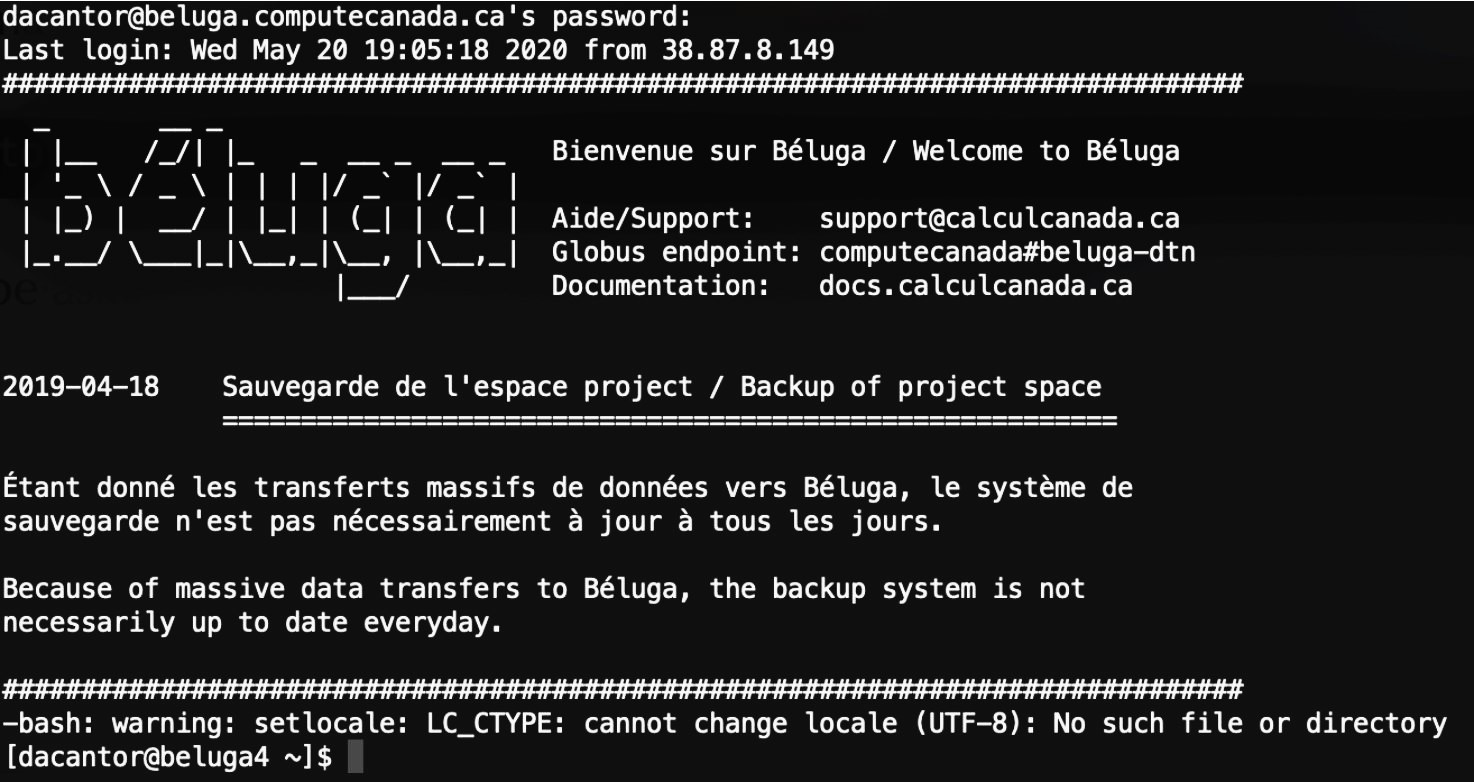
\includegraphics[width=1.\linewidth]{Screen_David2.jpg}
\end{figure}

\textbf{TIP:}
You may log into the server very frequently, so it may be annoying to write down each time the \texttt{ssh} line and your password. Install and use \texttt{sshpass} that will allow you to create a bash script that you can run each time you want to log-in. \\ 
No need to write down the \texttt{ssh} line or your password. Your script may look something like this:

\begin{figure}[H]
  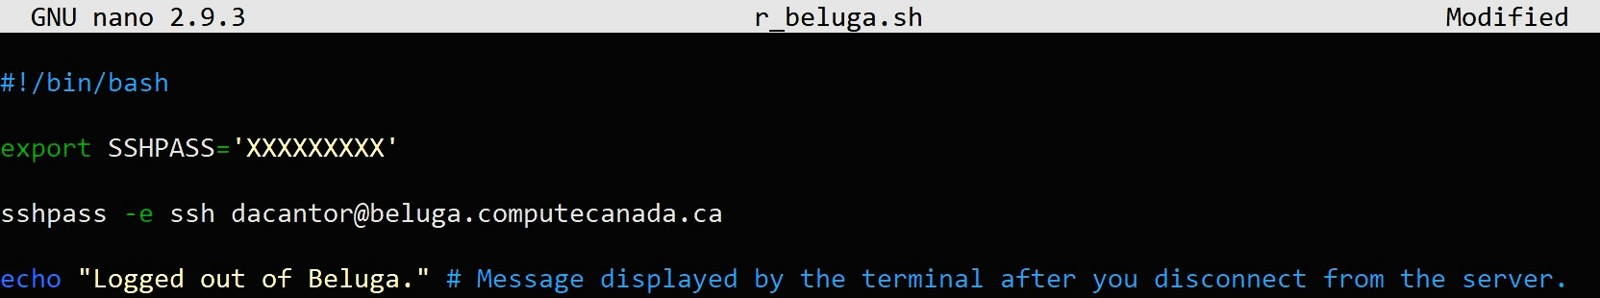
\includegraphics[width=1.\linewidth]{Screen_David3_modif.jpg}
\end{figure}

Then, in your terminal you only need to run \texttt{sh r\_beluga.sh} to get logged in the server.

Once logged in, you can see \texttt{ls} the structure of the folder you have access to by using the command:
\begin{figure}[H]
  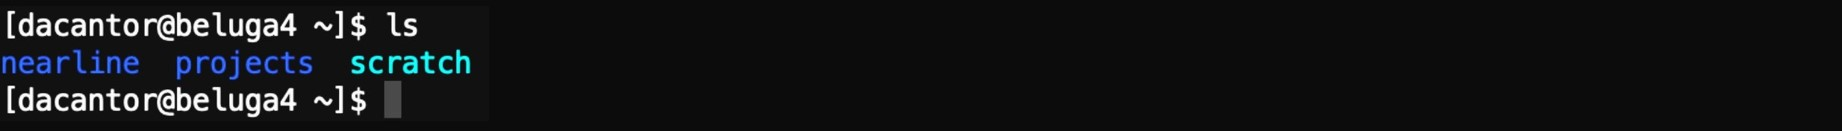
\includegraphics[width=1.\linewidth]{Screen_David4.jpg}
\end{figure}


\section*{Structures of the folders}
    
    1) \texttt{nearline}: Tape-like storage that does not consume our quotas of maximum storage. This folder allows you to store large files but it is quite slow compared to the others. Reading information from \texttt{nearline} can be time consuming as well (in the order of some minutes). \\
    
    2) \texttt{project}: Fast and daily backup storage of files. Files stored here are permanent and can be shared between the members of the group. The limit storage is 1 TB per group. \\ \break
    \uline{In this folder you should upload and install your version of LMGC90 or any other compiled code. However, you should not run your simulations here.} \\

    3) \texttt{scratch}: Large space for temporary storage of files during computations. The limit storage is 20 TB per user.
    Files of more than 60 days old are automatically deleted. So please, periodically check and download your files in scratch or you risk losing them permanently. \\ \break
    \uline{Your scripts for simulation (gen\_sample, command, and others) should be uploaded to your scratch and ran from there.}


\section*{Uploading and downloading data}
Among different methods, we recommend using \texttt{rsync} for uploading and downloading files to the server.

\textit{Example:} uploading LMGC90 to your \texttt{project} folder.

    - My \texttt{project} folder has the following path:
\begin{figure}[H]
  \centering
  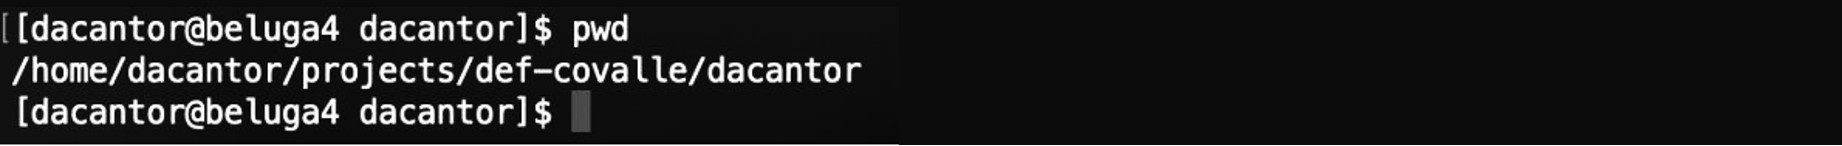
\includegraphics[width=1.\linewidth]{Screen_David5.jpg}
\end{figure}

In that location, create a new folder called \texttt{lmgc90\_v202005} (you can use another name if you want) using :
\begin{tcolorbox}
\texttt{[name@server name]\$ mkdir lmgc90\_202005}
\end{tcolorbox}

Then, you can get inside using :
\begin{tcolorbox}
\texttt{[name@server name]\$ cd lmgc90\_202005}
\end{tcolorbox}

Using \texttt{pwd}, you will get the path to that location:
\begin{figure}[H]
  \centering
  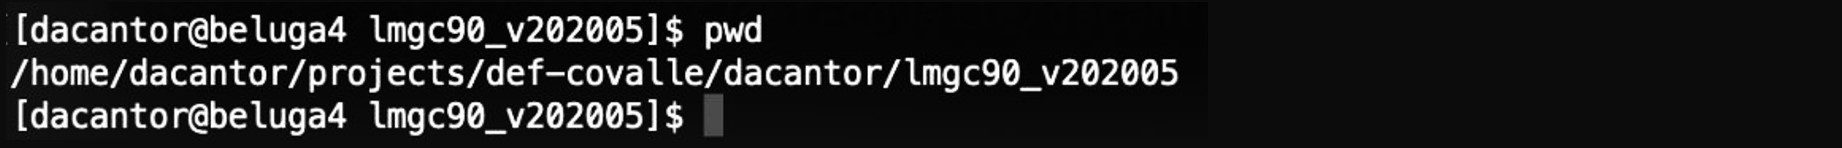
\includegraphics[width=1.\linewidth]{Screen_David6.jpg}
\end{figure}

Now, on your computer, using another window of terminal, go find the sources of LMGC90.

\textbf{NOTE:} Use one of the \texttt{version20XX.rc1} available in the \href{https://git-xen.lmgc.univ-montp2.fr/lmgc90/lmgc90_user/-/wikis/download_and_install}{\underline{website}}.

Upload your sources using the following command:
\begin{figure}[H]
  \centering
  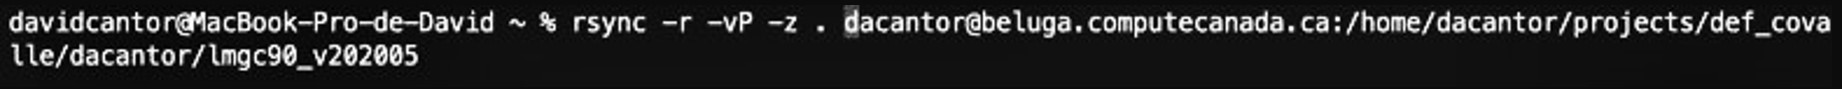
\includegraphics[width=1.\linewidth]{Screen_David7.jpg}
\end{figure}

To download files, for instance from a folder in your simulation folder \texttt{scratch}, you should refer to the following procedure.

First, go with a new window of terminal to the location you want ti download the files.

To know the location of your files in the server you can use \texttt{pdw}.
\begin{figure}[H]
  \centering
  
\includegraphics[width=1.\linewidth]{Screen_David8.jpg}
\end{figure}

In order to download the files in the folder \texttt{test\_run} use:
\begin{figure}[H]
  \centering
  
\includegraphics[width=1.\linewidth]{Screen_David9.jpg}
\end{figure}

You will to type down your password and the files will start to be downloaded.


\section*{Modules in the server}
The servers have a vast collection of softwares available. However, you have to explicitly define which are the modules you want to use. For instance, during the compilation of LMGC90 we need fortran, vtk, C++, and others.

The collection originally implemented on each cluster is defined by their standard environment. For a given \texttt{StdEnv} version, the implementation of LMGC90 needs a specific handling procedure.
\begin{itemize}
    \item \texttt{StdEnv/2018.3} is the standard environment originally implemented on both Béluga and Niagara.
    \item \texttt{StdEnv/2016.4} is the standard environment originally implemented on both Cedar and Graham.
\end{itemize}


First and foremost, we remind you that at any time and in any repertory of your server share you can access to the list of modules loaded by using the command:

\begin{tcolorbox}
\texttt{[name@server $\sim$]\$ module list}
\end{tcolorbox}

By doing so you must obtain an initial structure similar to the one displayed below. In particular, you must also be able to check, among a set of modules, which version of \texttt{StdEnv} is implicitly provided on the cluster you have chosen.
\begin{figure}[H]
  \centering
  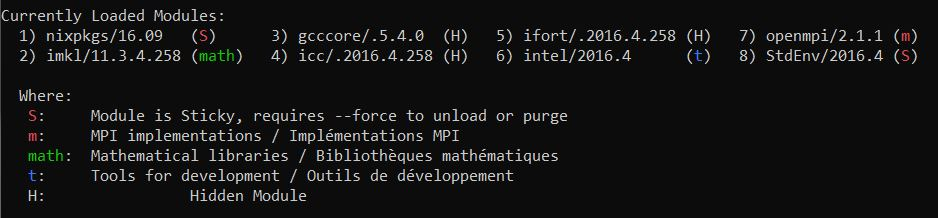
\includegraphics[width=1.\linewidth]{Screen1.jpg}
  \caption*{\textit{For instance, Béluga actually owns the} \texttt{StdEnv/2018.3}.}
\end{figure}
\vspace{-0.4cm}
At this point, you need to have uploaded LMGC90 data in a definite folder in such location:
\begin{tcolorbox}
\texttt{[name@server $\sim$]\$ cd projects/account\_name/name/lmgc90\_ 202005/}
\end{tcolorbox}

\vspace{0.5cm}
To load the modules that allow us to compile LMGC90, write the following line:
\begin{tcolorbox}
\texttt{[name@server lmgc90\_202005]\$ module purge \textcolor{red}{\textbf{A}}} 
\end{tcolorbox}
\vspace{0.5cm}

\begin{mdframed}
\vspace{0.5cm}
\ruleline{If you are using \textbf{Cedar} or \textbf{Graham}}

As previously stated, the compilation of LMGC90 requires specific modules but the root set \texttt{StdEnv/2016.4} is unable to give you access to the the needed packages. We are actually looking for its next update named \texttt{StdEnv/2018.3} (originally present on Béluga and Niagara) which you can load by overwriting the former environment:
\begin{tcolorbox}
\texttt{[name@server lmgc90\_202005]\$ module load StdEnv/2018.3 \textcolor{red}{\textbf{*}}} 
\end{tcolorbox}

\textbf{NOTE:} If the one above does not work, you may try:
\begin{tcolorbox}
\texttt{[name@server lmgc90\_202005]\$ module switch StdEnv/2016.4 StdEnv/2018.3 \textcolor{red}{\textbf{*}}} 
\end{tcolorbox}
\begin{figure}[H]
  \centering
  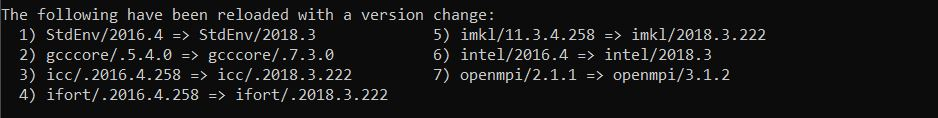
\includegraphics[width=1.\linewidth]{Screen2.jpg}
\end{figure}
\break

\end{mdframed}
\vspace{0.5cm}

Also, add:
\begin{tcolorbox}
\texttt{[name@server lmgc90\_202005]\$ module load vtk nixpkgs/16.09 gcc/7.3.0 hdf5 \textcolor{red}{\textbf{B}}} 
\end{tcolorbox}
\begin{figure}[H]
  \centering
  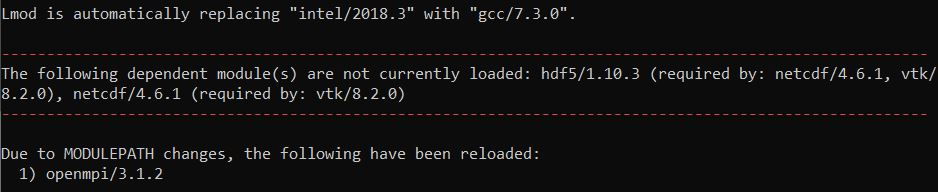
\includegraphics[width=1.\linewidth]{Screen3.jpg}
\end{figure}

Hopefully, you have obtained this type of response.
\begin{figure}[H]
  \centering
  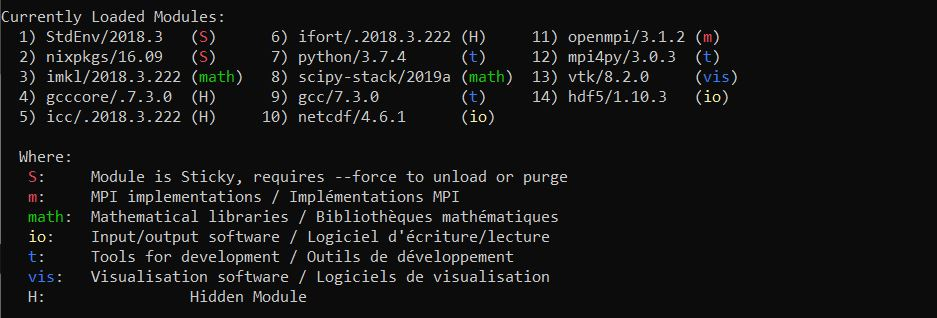
\includegraphics[width=1.\linewidth]{Screen4.jpg}
\end{figure}


You will need to run the same three lines \textcolor{red}{(\texttt{\textbf{A}}, \texttt{\textbf{B}} and if needed \texttt{\textbf{*}})} before running your simulations. In fact, you will systematically add them in each bash script from which we describe the structure later.


\section*{Installing LMGC90}
Adequate modules are now loaded. The compilation is done as explained below following the procedure given by the \href{https://git-xen.lmgc.univ-montp2.fr/lmgc90/lmgc90_user/-/wikis/Compilation}{\underline{LMGC90\_wiki page}}. 

Create a \texttt{build} folder with:
\begin{tcolorbox}
\texttt{[name@server lmgc90\_202005]\$ mkdir build} 
\end{tcolorbox}
Access to the \texttt{build}:
\begin{tcolorbox}
\texttt{[name@server lmgc90\_202005]\$ cd build}
\end{tcolorbox}
And compile with:
\begin{tcolorbox}
\texttt{[name@server build]\$ cmake .. -DMATLIB\_VERSION=none -DSPARSE\_LIBRARY=none} 
\end{tcolorbox}
\vspace{0.5cm}
Finally:
\begin{tcolorbox}
\texttt{[name@server build]\$ make} 
\end{tcolorbox}

The compilation went probably well, without raising any issue to your attention.


\section*{Running your simulations with the queuing assistant: SLURM}
You must use a queuing assistant called Slurm to run your simulations from one of the two clusters we are interested in.  We propose to work with a bash script. This same script will have to be in the folder of your simulation located somewhere in your \texttt{scratch}:
\begin{tcolorbox}
\texttt{[name@server $\sim$]\$ cd scratch/path/simu\_folder/}\\
\texttt{[name@server simu\_folder]\$ pwd}\\
\texttt{/home/name/scratch/path/simu\_folder}
\end{tcolorbox}

After you have uploaded the \texttt{DATBOX} folder and the \texttt{command.py} referring to your simulation in its folder, create the bash script with the command:
\begin{tcolorbox}
\texttt{[name@server simu\_folder]\$ nano script.sh} 
\end{tcolorbox}

In the nano editor you are then able to write a simple bash script from which we give you an example of structure below.
\begin{figure}[H]
  \centering
  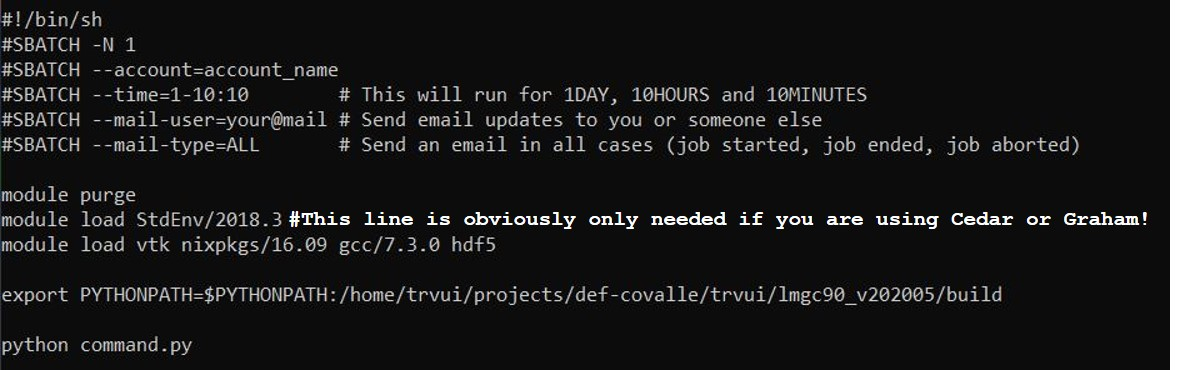
\includegraphics[width=1.\linewidth]{Screen5.jpg}
\end{figure}
\begin{itemize}
    \item The first line says that this is a bash script.
    \item Second line states that this belongs to the group \texttt{account\_name}.
    \item Third line states the duration of the simulation. In Béluga and Niagara the limit is set to 7 days, 28 days in Cedar and Graham.
    \item Fourth and fifth lines are optional but helpful. They will keep you updated of your simulation’s state by email so you do not have to keep an eye on it constantly.
    \item Then, the modules are purged and loaded as required.
    \item Next line states where the sources of LMGC90 are located.
    \item And finally, we run the simulation.
\end{itemize} 

Then, run it using:
\begin{tcolorbox}
\texttt{[name@server simu\_folder]\$ sbatch script.sh}
\end{tcolorbox}

To see all the jobs running at the same time use \texttt{squeue} (there are hundreds!).
To check the status of your jobs using \texttt{squeue} and your username as follows:
\begin{tcolorbox}
\texttt{[name@server $\sim$]\$ squeue -u name}
\end{tcolorbox}
To cancel a job use \texttt{scancel} and the number id of your job.
The outputs of your simulation will be located in a file called \texttt{slurm-XXX} with \texttt{XXX} the identifier of your job.

\textbf{NOTE:} Remember you should run your simulation in the \texttt{scratch} folder!


\section*{More options with SLURM}
Slurm gives you many options for running your simulations. You can run simulations in parallel if you compile the corresponding version of the code. When running simulations in parallel you should also explicitly state some variables in the Slurm script. We strongly recommend reading the options of running simulations in array or in parallel if necessary. 

Follow the instructions \href{https://docs.computecanada.ca/wiki/Running_jobs}{\underline{here}}.

\textbf{Important:} When running simulations in parallel remember to set in the Slurm script the following variables (besides those mentioned in the link above):
\begin{tcolorbox}
\texttt{export OMP\_SCHEDULE=STATIC} \\
\texttt{export OMP\_NUM\_THREADS=n} \\
\texttt{export OPENBLAS\_NUM\_THREADS=1} \\
\\
{where \texttt{n} is the number of threads you want to use (usually no more than the number of core available).}
\end{tcolorbox}

\end{document}